\documentclass[aspectratio=169]{beamer}
\usecolortheme{orchid}

\usetheme{boxes} % really plain and simple theme "boxes"
\usepackage[utf8]{inputenc}
\usepackage{caption}
\usepackage{graphicx}
\usepackage{multicol}
\usepackage{xcolor}
\usepackage{amsmath,amsthm,amssymb}
\usepackage[absolute,overlay]{textpos}
\usepackage{tikz}
\setbeamertemplate{footline}[frame number]

\newtheorem{question}{Question}

\setbeamertemplate{navigation symbols}{}
\title{Perspectives on Functions}
\author{Tyler Holden and Parker Glynn-Adey}

\begin{document}

\begin{frame}
	\maketitle
\end{frame}

\section{The MAT 135 Perspective}

\begin{frame}[t]
    \frametitle{135 Definition}
    A function $f(x)$ is an assignment of a real number $x$ to some other unique real number. 

    \begin{itemize}
        \item 
            \begin{minipage}[t]{0.4\textwidth}
                $f(x) = x^2$  
            \end{minipage}
            \begin{minipage}{0.4\textwidth}
                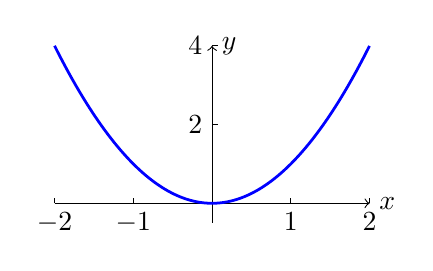
\begin{tikzpicture}[x=1cm, y=0.5cm]
                    \draw[->] (-2,0) -- (2,0) node[right]{$x$};
                    \draw[->] (0,-0.5) -- (0,4) node[right]{$y$};
                    \draw[line width=1pt, blue] plot[samples=101, domain=-2:2] (\x, {(\x)^2});

                    \foreach \x in {-2,-1,1,2} {
                        \draw (\x,0) node[below]{$\x$} --+ (0, 2pt);
                    }
                    \foreach \y in {2,4} {
                        \draw (0,\y) node[left]{$\y$} --+ (2pt,0);
                    }
                \end{tikzpicture}
            \end{minipage}

        \item 
            \begin{minipage}{0.4\textwidth}
                $f(x) = \sqrt{1-x^2}$
            \end{minipage}
            \begin{minipage}{0.4\textwidth}
                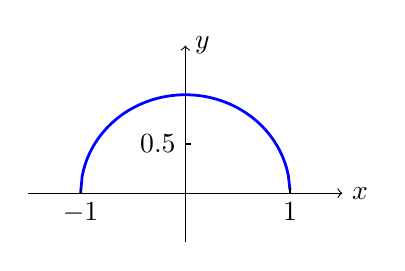
\begin{tikzpicture}[x=1.33cm, y=1.25cm]
                    \draw[->] (-1.5,0) -- (1.5,0) node[right]{$x$};
                    \draw[->] (0,-0.5) -- (0,1.5) node[right]{$y$};
                    \draw[line width=1pt, blue] plot[samples=131, domain=-1:1] (\x, {sqrt(1-(\x)^2)});
                        \foreach \x in {-1,1} {
                            \draw (\x,0) node[below]{$\x$} --+ (0, 2pt);
                        }
                        \foreach \y in {0.5} {
                            \draw (0,\y) node[left]{$\y$} --+ (2pt,0);
                        }
                \end{tikzpicture}
            \end{minipage}
    \end{itemize}
\end{frame}

\begin{frame}[t]

    \textbf{Definition:}
    The \emph{domain} of a function is the largest set on which the function is defined. The \emph{range} of a function is the set of all points which are witnessed by the function.

    \vfill


    \textbf{Example Question:} Find the domain and range of the function $f(x) = \displaystyle \frac1{\sqrt{1-x^2}}$.

    \vfill

    \textbf{Solution:} In the denominator we have a square root whose argument cannot be negative, so $1-x^2\geq 0$. Solving this gives $-1\leq x \leq 1$. This is the only restriction, so the domain is $[-1,1]$. For the range, note that every term of the function is non-negative, and it can never be zero, so $f(x) >0$ for any value of $x$. The function is smallest when the denominator is largest, which occurs when $x=0$, so the minimum of $f$ is $f(0) = 1$. As $x$ gets closer to $0$, the denominator becomes arbitrarily small, meaning that $f$ gets arbitrarily big, thus the range is $[1,\infty)$.


\end{frame}

\section{The MAT 137 Perspective}

\begin{frame}[t]
    \frametitle{137 Definition}
    Given two sets $A$ and $B$, a function is a map $f: A \to B$ such that $f(a) \in B$ for all $a \in A$. In this case, $A$ is said to be the \emph{domain}, while $B$ is said to be the \emph{codomain}.

    \begin{itemize}
        \item 
            \begin{minipage}{0.6\textwidth}
            Let $A = \{0,1,2\}$ and $B = \{a,b,c,d\}$, and define the function by the following map:
            \end{minipage}\qquad
            \begin{minipage}{0.2\textwidth}
                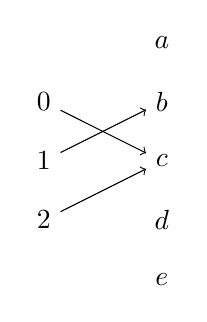
\begin{tikzpicture}[scale=0.75]
                    \foreach \y in {0,1,2} {
                        \pgfmathsetmacro\myval{int(2-\y)}
                        \node (\y) at (0,{\y+1}) {$\myval$};
                    }
                    \foreach \y/\mylab in {0/e, 1/d, 2/c, 3/b, 4/a} {
                        \node (\mylab) at (2,\y) {$\mylab$};
                    }

                    \draw[->](0) -- (c);
                    \draw[->](1) -- (b);
                    \draw[->](2) -- (c);
                \end{tikzpicture}
            \end{minipage}

        \item 
            \begin{minipage}{0.5\textwidth}
                Define $f: [0,1] \to \mathbb R$ by $f(x) = x^2$
            \end{minipage}
            \begin{minipage}{0.4\textwidth}
                 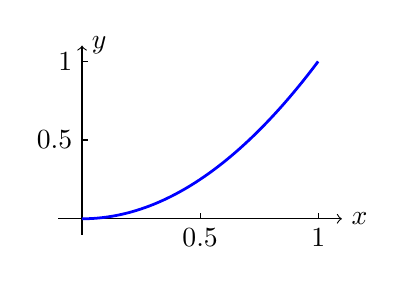
\begin{tikzpicture}[x=3cm, y=2cm]
                    \draw[->] (-0.1,0) -- (1.1,0) node[right]{$x$};
                    \draw[->] (0,-0.1) -- (0,1.1) node[right]{$y$};
                    \draw[line width=1pt, blue] plot[samples=101, domain=0:1] (\x, {(\x)^2});

                    \foreach \x in {0.5,1} {
                        \draw (\x,0) node[below]{$\x$} --+ (0, 2pt);
                    }
                    \foreach \y in {0.5,1} {
                        \draw (0,\y) node[left]{$\y$} --+ (2pt,0);
                    }
                \end{tikzpicture}
               
            \end{minipage}
    \end{itemize}
\end{frame}

\begin{frame}[t]
    \textbf{Definition:} A function $f: A \to B$ is said to be \emph{injective} if whenever $f(x) = f(y)$ then $x=y$. 

    \vfill

    \textbf{Example Question:} Suppose that $f: B \to C$ and $g: A \to B$ are functions such that $f \circ g: A \to C$ is injective. Show that $g$ is injective.

    \vfill

    \textbf{Solution:} We are told that $f\circ g$ is injective, which means that if $f(g(x)) = f(g(y))$ then $x=y$. We want to show that if $g(x) = g(y)$ then $x=y$. So suppose $g(x) = g(y)$, and apply $f$ to both sides, so that $f(g(x)) = f(g(y))$. But since $f\circ g$ is injective, it must be the case that $x=y$.

\end{frame}

\section{The MAT 157 Perspective}

\begin{frame}
    \frametitle{157 Definition(s)}
    
    \textbf{Definition:} The \emph{cartesian product} of two sets $A$ and $B$ is the set $A \times B = \{ (a,b): a \in A, b \in B\}$. 

    \vfill

    \textbf{Definition:} A \emph{binary relation} on the sets $A$ and $B$ is a subset $R \subseteq A \times B$.

    \vfill

    \textbf{Definition:} A function $f: A \to B$ is a binary relation $R$ on the sets $A$ and $B$ such that 
    \begin{enumerate}
        \item if $(x,y),(x,z) \in R$ then $y=z$. Here $A$ is the \emph{domain} and $B$ is the \emph{codomain};

        \item for every $x \in A$ there exists a $y \in B$ such that $(x,y) \in R$.
    \end{enumerate}

    \vfill

    \begin{itemize}
        \item For example, on the set $\{0,1,2\} \times \{a,b,c,d,e\}$ we can define a function via the relation $R = \{ (0,c), (1,b), (2,c)\}$. We often write this as $f(0) = c, f(1) = b, f(2) =c $.
        \item Define a function on $[0,1] \times \mathbb R$ by $R = \{ (x,x^2) : x \in [0,1]\}$, often written $f(x) = x^2$.
    \end{itemize}
\end{frame}

\begin{frame}[t]
    \textbf{Definition:} A function $f: B \to C$ is said to be \emph{monic} if whenever $g_1,g_2: A \to B$ satisfy $f \circ g_1 = f \circ g_2$ then $g_1=g_2$.

    \vfill

    \textbf{Example Question:} Show that a function is injective if and only if it is monic.

    \vfill

    \textbf{Solution:} Suppose that $f$ is a monomorphism, and that $b_1, b_2 \in B$ satisfy $f(b_1) = f(b_2)$. Define the constant functions $g_i: B \to B$ be the constant function $g_i(x) = b_i$. Now $f(g_1(x)) = f(b_1) = f(b_2) = f(g_2(x))$ for all $x \in B$, so by assumption $g_1(x) = g_2(x)$ for all $x \in B$, which in turn shows that $b_1 = b_2$.

        Conversely, suppose that $f$ is injective. Injective functions are left-invertible, so choose one such inverse $h : C \to B$ such that $h \circ f = \operatorname{id}_B$. Let $g_1,g_2: A \to B$ be any to functions such that $f\circ g_1 = f\circ g_2$, and post-compose by $h$ to get
        \begin{align*}
            h \circ (f \circ g_1) 
                &= (h \circ f) \circ g_1 = \operatorname{id}_B \circ g_1 = g_1 \\
                &= h \circ (f \circ g_2) & \text{by assumption} \\
                & = (h \circ f) \circ g_2 = \operatorname{id}_B \circ g_2 = g_2.
        \end{align*}
        This shows that $g_1 = g_2$, allowing us to conclude that $f$ is a monomorphism as required.

\end{frame}

\end{document}
